\documentclass[a4paper,10pt]{article}
\usepackage[utf8x]{inputenc}
\usepackage{array}
\usepackage{graphicx}
\usepackage{float}
\usepackage{color}
\usepackage{alltt}
\usepackage[T1]{fontenc}
\usepackage{ae,aecompl}

%opening
\title{Context Free General Top Down Parsing in Cubic Time}
\author{Arnold Lankamp}

\begin{document}

\maketitle

\begin{abstract}

In this article we will describe our general top-down parsing algorithm. Our intent with this algorithm is to develop something that is both easy to comprehend and performs well on any grammar. The user should not be required to refactor a grammar to enable the parser to complete within an acceptable amout of time. Additionally, it should not be hard to grasp what is going on under the hood, nor should it be complicated to create an implementation of this algorithm.

It sounds fairly ambitious, but we managed it. We created a general parsing algorithm that is both easy to understand and can compete with any other general parsing algorithm out there in terms of scalability and performance.

\end{abstract}

\section{Introduction}

If the abstract did not catch your attention yet, here are some highlights:
\begin{itemize}
 \setlength{\itemsep}{0pt}
 \setlength{\parskip}{0pt}
 \setlength{\parsep}{0pt}
 
 \item Worst-case cubic space and time bounds with respect to the length of the input string.
 \item Worst-case linear scaling relative to the size of the grammar.
 \item Linear performance on LL and LR grammars.
 \item No performance hit for rules that are not left factored.
 \item No penalty for being scannerless.
 \item Low stack activity.
 \item Generating or hand crafting the recognizer / parser code is trivial.
 \item Parse traces are easy to visualize.
\end{itemize}

For our parsing algorithm we choose for a top-down approach, as it is more in-line with human thinking then bottom-up. This makes the algorithm and implementation easier to comprehend. Ultimately it should also make its usage simpler, since grammars can more easily be converted to input for the parser; the translation is one-on-one and does not require any extra work, unlike what is necessary when generating parse tables. Nor will it ever explode in size, which parse tables potentially could. Lastly, top-down parsers can also generate understandable error reports more easily, which is a very welcome feature.

However, general top-down parsers do have the image of being slower than general bottom-up parsers. Mostly because they tend to perform poorly on non-left-factored grammars. Additionally, they usually try to recover from parse errors by back-tracking, which does not scale well, especially in absence of memorization. Our algorithm and implementation do not suffer from any of these problems.

We call our parser, the Scannerless General Top Down Binary Forest Parser or SGTDBF.

\section{Recognizer}

First we will discuss the algorithm for the recognizer, for simplicity's sake. Further on in this article we will explain how the recognizer can be extended to become a parser.

\subsection{GSS}

As is common in general parsing, we use a kind of Graph Structured Stack (GSS). In our case we generate a stack node with a unique identifier for every item in the grammar. For example; if take the following grammar: $S\,::=\,AB\,|\,BA,\,A\,::=\,a,\,B\,::=\,b$, we would assign these identifiers as follows: $.S$(-1), $.AB$(0), $A.B$(1), $.BA$(2), $B.A$(3), $.a$(4) and $.b$(5). These identifiers are needed to be able to handle the sharing of GSS nodes correctly, so regardless whether or not comparable items exist, they should not be merged. Each stack node consists of this identifier, edges back to their `parents' in the graph, information about its `right neighbour' in the production and the location in the input string it is associated with. Each stack node is unique for each identifier, location combination.

\subsection{Basic algorithm}

\begin{enumerate}
 \setlength{\itemsep}{0pt}
 \setlength{\parskip}{0pt}
 \setlength{\parsep}{0pt}

 \item Expand the left most node of every production that did not match anything yet on all stacks, until no stacks can be expanded anymore (i.e. they all have a terminal at the bottom).
 \item Match all nodes on the bottom of the stacks to the input. Reduce the ones that match, remove the ones that do not.
 \item Reduce the nodes on all stacks that matched something and have them queue the `next' node in the production they are part of where applicable, until no reductions are possible anymore.
 \item If there are nodes queued for expansion go to 1.
 \item If the end of the input has been reached and we have at least one derivation for one of the start symbols we are successful; otherwise recognition failed.
\end{enumerate}

\pagebreak
\subsection{Pseudocode}

{\small
\begin{verbatim}
main(){
  toExpandSet.add('startNode');
  expand();
  
  while(hasMoreStacksToReduce()){
    toReduceSet = getStacksToReduce();
    if(shiftedLevel){ // Nullable related sharing
      expandedSet.clear();
      reducedStore.clear();
    }
    
    reduce();
    expand();
  }
  
  if(endOfInputHasNotBeenReached()) error;
}
\end{verbatim}
}

This is the main function of the recognizer. It starts with building the stacks for the first level, by queuing the `start node' and expanding it. Once it has done so it will keep alternating between reducing and expanding until there are no more stacks left alive. At the start of each iteration we check whether or not we need another iteration in the current level or need to shift to the next one. In case we shifted we need to discard all level specific data from the previous level. This behaviour is necessary to be able to handle nullables properly.

{\small
\begin{verbatim}
expand(){
  while(node <- toExpandSet){
    if(node.isTerminalOrEpsilon()){
      if(node.match(input)){
        toReduceSet.add(node);
      }
    }else{
      expandedSet.add(node);
      
      for(childNode <- getChildren(node)){
        if(expandedSet.contains(childNode)){
          childNode = expandedSet.get(childNode);
        }else{
          toExpandSet.add(childNode);
        }
        childNode.addEdge(node);
      }
    }
  }
}
\end{verbatim}
}

This is the expand loop. It will iterate over the {\bf toExpandSet} until there are no more stacks queued for expansion. While expanding we check the type of the node we are handling. If the node is a terminal or an epsilon it needs to match the input (epsilons naturally always match). If it matches, it is added to the {\bf toReduceSet}; otherwise we discard it, causing the stack it was associated with to die of. If the node is a non-terminal, we retrieve its `children', add edges from these children to the current node and queue them for expansion (if not done so already), by adding them to the {\bf toExpandSet}. In case a child node is present in the {\bf expandedSet} it has already been expanded and will not be queued again. Additionally we will need to add an edge to the equivalent node from the {\bf expandedSet} instead of the current child node, for sharing purposes.

{\small
\begin{verbatim}
reduce(){
  while(node <- toReduceSet){
    if(node.lastInProduction()){
      for(edgeLevel <- node.edgesPerLevel){
        if(reducedStore.notContains(edgeLevel.getOne())){
          for(edges <- edgeLevel){
            toReduceSet.add(parent);
          }
          
          reducedStore.add(node);
        }
      }
    }else if(node.hasNext()){
      next = node.next;
      
      if(toExpandSet.notContains(next)){ // Sharing
        next = toExpandSet.get(next);
      }else{
        toExpandSet.add(next);
      }
      next.addEdges(node.edges);
    }
  }
}
\end{verbatim}
}

This is the reduce loop. It will iterate over the {\bf toReduceSet} until there are no more stacks queued for reduction. When a node is being reduced, one of two things can happen. Either it is the last node in the production and we need to queue this node's `parents' for reduction (if not reduced of queued for reduction already), by adding them to the {\bf toReduceSet}. Otherwise we need to move to the `next' node in the production and queue this `next' node for expansion and transfer all edges from this node to the next. In case the `next' node has already been scheduled for expansion we need to retrieve the equivalent `next' node from the {\bf toExpandSet} and add the edges to that node instead, for sharing purposes.

The edges are grouped by level. This level indicates the start location of the node the edge points to. To check whether or not the parents of a node need to be queued for reduction, we get one of the edges from each {\bf edgeLevel} and check if the node this edge points to has been reduced yet or not. If a node has not been reduced yet, we queue all of the nodes that are pointed to from edges in that {\bf edgeLevel} for reduction; otherwise we do not. This will work correctly since every node containing a non-terminal of the same sort always has exactly the same parents in the same level. Note that for the recognizer this behaviour is not a necessity, but an optimization (which reduces the number of edge visits by a factor between one and the number of non-terminals in the grammar). However for the parser this behaviour is required to achieve proper sharing in the resulting trees (in an uncomplicated and fast way).

The {\bf reducedStore} is a dual layered data structure. The first layer is indexed by the {\bf start position} of the node and the second layer by the sort name of the non-terminal in the node. Since the recognizer algorithm assumes it is level synchronized, the {\bf reducedStore} can contain a variant for every non-terminal for each possible substring up until the current location. This {\bf reducedStore} is necessary to keep track of which nodes have or have not been reduced yet.

Note that the first layer of the {\bf reducedStore} needs to be implemented as an array or table with O(1) look-up time; otherwise it is not possible to guarantee worst-case cubic time complexity.

\subsection{Correctness}

In this section we will go into detail on some special cases that deserve some extra attention.

\subsubsection{Left recursion}
First of all, left recursion. Normal top-down parsers cannot handle grammar rules containing left recursion, since they can keep expanding left recursive rules indefinitely, preventing implementations of these kind algorithms from terminating. Because we introduce sharing into the GSS, which leads to automatic terminalization of all these rules, this undesirable behaviour is prevented from manifesting. By terminalization we mean that the expansion phase converges to a point at which each stack has a terminal at the bottom and thus cannot be expanded further. For example, if we take the grammar:\\
$S ::= A$\\
$A ::= Aa\,|\,a$\\
We would expand these rules in the following way:
\begin{figure}[H]
\centering
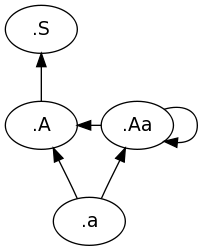
\includegraphics[scale=0.5]{left-recursive.png}
\caption{GSS representation of an expanded left-recursive grammar.}
\end{figure}
As can be seen a cycle is added to the graph, since $.Aa$ is, in a way, a child of itself. To see how left recursive grammars work in action see section \ref{sec:tracesLeftRecusive}.

\subsubsection{Cycles}
TODO: Add text.\\
-Sharing fixes everything.

\subsubsection{Breadth-first vs depth-first}
Another requirement of the algorithm, of which the reason may not be immediately obvious, is that it needs to be level synchronized. We will demonstrate why the depth-first sibling does not work correctly without modification and why this modification would break the cubic time bound, by means of an example. Consider the following grammar: $S ::= SSS\,|\,a\,|\,aa$. Now imagine we are somewhere in the middle of recognizing an input string containing a number of $a$'s; currently we are recognizing $SS.S$, which matches with one $a$. The preceding items that belong to this production, $.SSS$ and $S.SS$ both recognized one $a$ as well. Causing $S(S(a),S(a),S(a))$ to be reduced at this location. We progress a bit more and are now recognizing $.SSS$ at a location that is one character earlier in the input string as the other $.SSS$ we recognized before; this time it matches $aa$. Since we now end up at a $S.SS$ node at a location where it was already recognized, we do not progress further; this node needs to be shared, otherwise we would do duplicate work, breaking the cubic time bound. However, in the scheme we are using, sharing this node means we stop recognizing the current derivation, preventing reductions from being executed. Which in this case will mean that we fail to recognize the derivation $S(S(aa),S(a),S(a))$ at the current location. If we would be using a different grammar it could even cause recognition to fail entirely because of this behaviour.

This problem could be solved by tracing forward through the production, gathering any potential missing derivation(s) and executing reductions where necessary. However this would cause the algortihm to become unbound polynomial in time, since it would lead us to `touch' nodes $N^{(productionLength+1)}$ times in the worst-case.

In our opinion the solution for this problem is both to complicated and, above all, unnecessary. Since our algorithm is breadth-first, we will never have stacks running ahead of others, eliminating the possibility of this behaviour popping-up. We do need extra iterations within the same level to handle nullables, but this is only a problem for the parser, which needs to keep track of hidden right recursion. We will cover the handling of hidden right recursion in the parser in section \ref{sec:parserCorrectness}.

\subsection{From grammar to code}

Converting a grammar to a recognizer or parser, either by hand writing or generating it, is relatively straight forward. All that is needed is a direct translation from the grammar rules to either functions or a table like data structure. Basically the recognizer just needs to know what alternatives are associated with each left-hand-side. In case we are generating code, this would mean that we need one function per non-terminal sort, which contains logic that informs the recognizer about what alternatives should be expected.

Since the mapping between the original grammar and the code or table is one-on-one, it is possible to implement or edit it by hand without much effort. Another advantage is that, in combination with the top-down-ness of our algorithm, it makes tracing errors in a grammar easier; if you would like to know why something does not match at a certain position, you can just go through it with a debugger to see what happens (your degree of success naturally depends on the amount of stacks that are alive at the moment you are trying to observe, but at least the possibility to do so exists).

\subsection{Example traces}

To illustrate how the recognizer works in action, we constructed some example traces using various grammars to give an impression.

\subsubsection{Straight forward}
First we will take a look at a simple non-ambiguous grammar:\\
$S\,::=\,AB$\\
$A\,::=\,a$\\
$B\,::=\,b$\\
input = $ab$

\begin{enumerate}
 \setlength{\itemsep}{0pt}
 \setlength{\parskip}{0pt}
 \setlength{\parsep}{0pt}
 
 \item expand $.S$
 \item expect $.AB$
 \item expand $.AB$
 \item expect $.a$; $.a$ matches
 \item reduce $a.$ and follow edge to $.AB$
 \item move from $.AB$ to $A.B$
 \item expand $A.B$
 \item expect $.b$, $.b$ matches
 \item reduce $b.$ follow edge to $A.B$
 \item reduce $AB.$ and follow edge to $.S$
 \item parse for $S.$ is complete 
\end{enumerate}
This one is easy to follow and does not really need any additional explanation.

\subsubsection{Left recursive}
\label{sec:tracesLeftRecusive}
Next up is a grammar containing a left-recursive rule:\\
$S\,::=\,A$\\
$A\,::=\,Aa\,|\,a$\\
input = $aaa$

\begin{enumerate}
 \setlength{\itemsep}{0pt}
 \setlength{\parskip}{0pt}
 \setlength{\parsep}{0pt}
 
 \item expand $.S$
 \item expect $.A$
 \item expand $.A$
 \item expect $.Aa$ and $.a$; $.a$ matches
 \item expand $.A$ $\Rightarrow$ $.A$ shared
 \item reduce $a.$ and follow edges to $.A$ and $.Aa$
 \item reduce $A.$ and follow edges to $.S$
 \item parse for $S.$ is incomplete and is discarded
 \item move from $.Aa$ to $A.a$; $A.a$ matches
 \item reduce $Aa.$ and follow edges to $.A$ and $.Aa$
 \item reduce $A.$ and follow edges to $.S$
 \item parse for $S.$ is incomplete and is discarded
 \item move from $.Aa$ to $A.a$; $A.a$ matches
 \item reduce $Aa.$ and follow edges to $.A$ and $.Aa$
 \item reduce $A.$ and follow edges to $.S$
 \item parse for $S.$ is complete
 \item move from $.Aa$ to $A.a$; $A.a$ does not match since EOI has already been reached
\end{enumerate}
As one can see, when expanding $.A$ for the second time (at 5), sharing is detected causing a cycle to be added to the GSS. Reductions of $Aa.$ follow the edge back to $.Aa$ which will move to $A.a$; this will lead to one $a$ being matched at each `iteration' and ultimately consuming all of them.

\subsection{Worst-case complexity}
\label{subsec:recognizerComplexity}

We are designing a parsing algorithm that is intented to scale as well as is possible, regardless of the input grammar. For this reason, the recognizer must not break the cubic time bound. Here we will prove that we remain within this bound.

Since the GSS only contains nodes that we expect to `encounter', there are at most $O(N)$ of them; where $N$ is the number of characters in the input string. Each node only has one edge to each of its possible parents per level and there are $N$ levels, so there are at most $O(N)$ edges per node. In the worst-case there are $N$ times $O(N)$ nodes that match a substring that ends at the `current' level. When moving to the `next' node in the production, all edges of these nodes need to be carried over. Since these sets of edges need to be merged, the time this operation needs to complete is equal to the number of levels before (and including) the `current' level (so $N$ at most). So this operation will execute in $O(N^3)$ time at most in the worst-case.

Reducing consumes $O(N^3)$ time in the worst-case as well. Each of the $O(N^2)$ edges is associated with one reduction. The check whether or not each of the parents still needs to be reduced, is an operation that completes in $O(1)$ time. However we do need to visit the edge to this parent to be able to determine who this parent is. This happens $N$ times per edge at most. So each edge is visited $O(N^3)$ times at most.

This means that the algorithm remains within cubic time bounds in worst-case scenarios.

\section{Parser}

\subsection{Parse forest}

To represent the parse forest we use a format that was especially designed for this parser, to ensure worst-case behaviour remains within cubic space and time bounds. We call it `deflattenized', for lack of a better description. While its purpose is similar to binarized SPPFs, its implementation is somewhat different.

The parse forest consists of nodes. Every node in the forest contains a result and a set of prefixes. Each results represents a substring for a certain symbol. In case this symbol is a non-terminal, this result contains one or more references to alternative representations of the substring it denotes. If the symbol is a terminal, it will just represent that specific terminal. The set of prefixes contained in the node hold all possible alternatives for the preceding item in the production. (Naturally this set is empty for the node containing results for the first item in the production). A prefix only consists of a reference to a node. If one traces all possible paths through this representation of a production to the start, you will get all alternatives for this production of the substring it represents.

Note however, that the parser forest contains an exact representation of what the parser recognized. This means it can contains cycles.

\subsubsection{Example}
To give an idea of what a typical parse forest would look like we will give an example using the following grammar:\\
$S\,::=\,AAA$\\
$A\,::=\,a\,|\,aa$\\
input = $aaaa$

\begin{figure}[H]
\centering
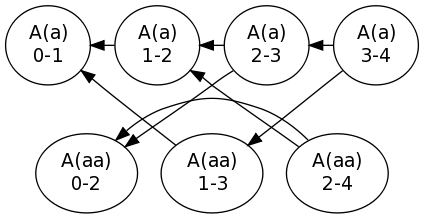
\includegraphics[width=0.5\textwidth]{a_aa-forest.png}
\caption{A visual representation of the parse forest, showing all alternatives for the given input string. The numbers indicate the start and end position of the matched substring.}
\end{figure}

In the figure above we see the parse forest. It illustrates how the parse results are stored in memory.

To show how we can obtain all possible derivations from this parse forest, we will list them in the table below; which relates each path through the forest to a derivation.

\begin{table}[H]
\centering
\begin{tabular}{ p{15em} p{15em} }
Derivation & Forest path\\
\hline
S(A(a),A(a),A(aa)) & $A0$-$1$ $\leftarrow$ $A1$-$2$ $\leftarrow$ $A2$-$4$\\
S(A(a),A(aa),A(a)) & $A0$-$1$ $\leftarrow$ $A1$-$3$ $\leftarrow$ $A3$-$4$\\
S(A(aa),A(a),A(a)) & $A0$-$2$ $\leftarrow$ $A2$-$3$ $\leftarrow$ $A3$-$4$
\end{tabular}
\caption{A flattened representation of the parse forest, listing all derivations.}
\end{table}

\subsection{Psuedocode}

Augmenting our recognizer with parse tree construction code is trivial. Only a few minor adjustments are needed. Relevant pieces of code, containing changes or additions, are highlighted in italic.

\pagebreak
{\small
\begin{alltt}
main()\{
  toExpandSet.add('startNode');
  expand();
  
  while(hasMoreStacksToReduce())\{
    toReduceSet = getStacksToReduce();
    if(shiftedLevel)\{ // Nullable related sharing
      expandedSet.clear();\textit{
      resultStore.clear();}
    \}
    
    reduce();
    expand();
  \}
  
  if(endOfInputHasNotBeenReached()) error;
  \textit{
  return resultStore.get('startNode');}
\}
\end{alltt}
}

The only things that need to be changed in the main function to transform the recognizer into a parser are the returning of the final result (if not in error) and replacing the {\bf reducedStore} by {\bf resultStore}. The {\bf resultStore} is similar to the {\bf reducedStore}, except that it also contains the result associated with the non-terminal sorts in the store.

{\small
\begin{alltt}
expand()\{
  while(node <- toExpandSet)\{
    if(node.isTerminalOrEpsilon())\{
      if(node.match(input))\{
        toReduceSet.add(node);
      \}
    \}else\{
      expandedSet.add(node);
      
      for(childNode <- getChildren(node))\{
        if(expandedSet.contains(childNode))\{
          childNode = expandedSet.get(childNode);
        \}else\{
          toExpandSet.add(childNode);
        \}
        childNode.addEdge(node);
      \}
    \}
  \}
\}
\end{alltt}
}

The expansion code does not need to change in any way, since it does not deal with parse results. But we still list it here for completeness.

\pagebreak
{\small
\begin{alltt}
reduce()\{
  while(node <- toReduceSet)\{
    if(node.lastInProduction())\{
      for(edgesLevel <- node.edgesPerLevel)\{\textit{
        if(resultStore.contains(edgesLevel.getOne()))\{
          result = resultStore.get(edgesLevel.getOne());
        \}else\{
          result = createResult(edgesLevel.getOne());
          for(edges <- edgesLevel)\{
            toReduceSet.add(parent);
          \}
        \}
        result.
            addAlternative(node.prefixes, node.results);}
      \}
    \}else if(node.hasNext())\{
      next = node.next;
      
      if(expandedSet.notContains(next))\{ // Sharing
        next = expandedSet.get(next);
      \}else\{
        toExpandSet.add(next);
      \}
      next.addEdges(node.edges);\textit{
      next.updatePrefixes(node.prefixes, resultStore.get(node));}
    \}
  \}
\}
\end{alltt}
}

The reduce code does need to be modified. Basically two things need to be added.

First of all the storing of results. We need to create (at most) one {\bf result} per sort of non-terminal for each matched substring; no more then that. In the recognizer code we used the {\bf reducedStore} for a similar purpose. Here it is replaced by the {\bf resultStore}, which basically is the same thing, but with results associated with the non-terminal sorts in the store.

Secondly we need to add {\bf prefixes} to the nodes that are being queued for expansion when we are moving to the {\bf next} node in the production. We do this by creating a new prefix using the prefix of the current node and its result and adding it to the {\bf next} node. We add the prefixes to GSS nodes for convenience reasons; regardless of where the result(s) of the node end, they will always share the same prefix. By adding the prefixes to the GSS nodes they are easy to retrieve; all these nodes need is a collection that holds all the prefixes for it, grouped by the start location of the production.

{\small
\begin{alltt}
\textit{createResult(node)\{
  result = allocateResult(node.startLocation, node.sort);
  resultStore.add(result);
  return result;
\}}
\end{alltt}
}

\pagebreak
We also need a function for creating {\bf results}. Every time a result is created we need to add it to the {\bf resultStore}. The {\bf start position} and non-terminal {\bf sort} of the given node are used as keys. Like the {\bf reducedStore} the {\bf resultStore} is a dual layered datastructure, where the first layer is indexed using the {\bf start position} of the node and the second layer by the non-terminal {\bf sort} the node represents.

\subsection{Correctness}
\label{sec:parserCorrectness}

Since the conversion of our recognizer to a parser is so trivial, the parser is as correct as the recognizer. The only difference, as mentioned before, is the handling of hidden right recursion.

\subsubsection{Hidden right recursion}
The reason for complications related to hidden right recursion is that multiple iterations within the same level are possible. This could cause results to `go missing'. The only thing that needs to be done to fix this, is to check whether or not the next node is the last node in the production and is a nullable with results, in case the current node is also a nullable. If this is the case we need to construct the necessary result nodes and add them to their corresponding parents. This is a fairly general description of how to solve it, since the best way to handle this issue may differ per implementation. All that is needed is that the implementor is aware of this issue and takes it under consideration.

\subsection{Worst-case complexity}
We looked at the worst-case behaviour of the recognizer in section \ref{subsec:recognizerComplexity} and proved that is does not break the cubic time bound. For the parser to be able to make the same guarantee, the size of the parse forest must be, at most, cubic in the length of the input. The reason for this, is that it is impossible to construct a greater then cubic parse forest in a cubic amount of time. Here we will prove that we do not break this space bound.

Every node in the tree is identified by the substring its contained result represents and its prefixes. There can be only one result per substring, this means there are at most $O(N^2)$ results. The prefix sets are identified by the start and end position of the substring they represent, so there are at most $O(N^2)$ of them. Each prefix set can contain up to $N$ different prefixes, which all denote the same substring; at most one per location (before the current location) in the input string. So there are at most $O(N^3)$ prefixes. The number of unique nodes is determined by multiplying the number of results by the number of prefix sets. However, since a prefix set can only be matched in a node, together with a result that starts at the same position as the prefix ends each prefix set can be associated with $O(N)$ different results at most. Hence the number of unique nodes is limited to $O(N^3)$, making the parse forest $O(N^3)$ worst-case. Note that in the implementation all prefix sets are shared regardless of the end position of the node they are matched to; this has no effect on worst-case behaviour, but does improve performance and decreases memory usage.

\subsubsection{Worst-case statistics}
We have already theoreticly proven that the recognizer / parser will be $O(N^3)$ in the worst-case. In this section we will show that in practice this is indeed the case.

We will give an overview of the most relevant parser statistics for the following grammar:\\
$S\,::=\,SSS\,|\,SS\,|\,a$\\
input = $a * 2$ to $a * 10$, $a * 50$, $a * 100$, $a * 200$, $a * 300$, $a * 400$ and $a * 500$

\begin{table}[H]
\centering
\begin{tabular}{ | p{7ex} | p{7ex} | p{7ex} | p{10ex} | p{8ex} | p{10ex} | p{10ex} | }
  \hline
  Input & GSS & Edges & Edge & Results & Prefixes & Forest \\
  length & nodes & & visits & & & nodes \\
  \hline
  2 & 9 & 7 & 6 & 3 & 1 & 2 \\
  3 & 13 & 10 & 15 & 6 & 4 & 8 \\
  4 & 17 & 13 & 31 & 10 & 10 & 20 \\
  5 & 21 & 16 & 56 & 15 & 20 & 40 \\
  6 & 25 & 19 & 92 & 21 & 35 & 70 \\
  7 & 29 & 22 & 141 & 28 & 56 & 102 \\
  8 & 33 & 25 & 205 & 36 & 84 & 168 \\
  9 & 37 & 28 & 286 & 45 & 120 & 240 \\
  10 & 41 & 31 & 386 & 55 & 165 & 330 \\
  \hline
  50 & 201 & 151 & 42926 & 1275 & 20825 & 41650 \\
  100 & 401 & 301 & 338351 & 5050 & 166650 & 333300 \\
  200 & 801 & 601 & 2686701 & 20100 & 1333300 & 2666600 \\
  300 & 1201 & 901 & 9045051 & 45150 & 4499950 & 8999900 \\
  400 & 1601 & 1201 & 21413401 & 80200 & 10666600 & 21333200 \\
  500 & 2001 & 1501 & 41791751 & 125250 & 20833250 & 41666500 \\
  \hline
\end{tabular}
\caption{Worst-case parser statistics (for the fully optimized version).}
\end{table}

In the table above we can see how the different components in the parse forest increase with respect to the length of the input string. Note however that all optimizations mentioned in chapter \ref{chap:optimizations} were enabled while gathering these statistics; most notably edge sharing (\ref{sec:edgeOptimizations}) and GSS prefix-sharing (\ref{sec:prefixSharing}).

The number of GSS nodes and number of edges scale linear with respect to the length of the input string. The number of edge visits remains within the cubic bound and is only slightly higher then the number of result nodes. The `extra' visits are for failed parse results, one for each location in the input string squared. This means the number of edge visits is as low as they can possibly be; meaning we can conclude that an algorithm with less stack activity is impossible to concieve.

Looking at the parse tree related statistics we can see that the number of results increases by $N$ for every extra character in the input string. Which is because the number of results is equal to the number of different substrings in the input, in this case. As can be observed, the number of prefixes and number of nodes remains within cubic bounds for this worst-case example.

\subsubsection{Flattening}
Optionally it is possible to output a flattened version of the parse forest at the user's request. Naturally the size of this parse forest will be unbound polynomial relative to the length of the input, in the worst-case. Although, in practice this unlikely to happen; moreso since filtering can be done during parsing and flattening, making it improbable that many ambiguities remain in the final tree, in the general case. We will discuss filtering in chapter \ref{chap:filtering}.

One might wonder why, in case one flattens the parse forest afterwards, using the `deflattenized' version as internal representation would be advantageous. The reason for this is that it enables us to guarantee that both the recognition and parse phases will always be cubic with respect to the length of the input in the worst-case. If we would not use the `deflattenized' representation we would not be able to make this guarantee for the parse phase. The consequence of this is that it may make the parsing of input for certain grammars unfeasible. While it may be feasible to flatten the final parse result in these cases. The main reason that this is a possibility is because of the stravation of incomplete parse results; either ones that died because they failed to match the input further down the line or because they were filtered. In both cases it will prevent their results from being added to the parse forest as alternatives. This means the final parse result will likely have less nodes in it then there are constructed in total while parsing, reducing the amount of nodes the flattener has to touch.

\section{Extended capabilities}

To improve the usefulness of the parser on real grammars a few additional features were added. Namely support for lists, optionals and location related features is added. In this chapter we will discuss how these features can be intergrated into our algorithm and implementation.

\subsection{Lists}

List, separated lists and optionals are handled in a similar way, because in essense they are the same. However their semantics are slightly different; separated lists are lists with extra symbols between their elements and optionals are star-lists with one element at most; from here on out we will refer to all of these simply as `lists'.

Often lists are implemented by adding extra `virtual' rules to the grammar. For example $S\,::=\,A+,\,A\,::=\,a$ can be parsed like a `normal' grammar, if we add the rule $A+\,::=\,AA+\,|\,A$. The advantage of this approach is that the parser does not need to be modified. On the other hand, we always get a binarized version of the list as a result, that uses these imaginary productions, which may not be what we wanted. Additionally, because an extra rule is inserted into the grammar we need more GSS nodes to be able to parse the list.

Our approach involves special casing the handling of lists, by introducing additional types of GSS nodes that contain knowledge about how they need to be expanded. For example to expand the star-list $A*$, it would queue an $\epsilon$ and a $A$ non-terminal GSS node; this $A$ GSS node has a `next' pointer to itself and is marked as last node in the `production' (see figure below). One could view this construction as a GSS node with a kind of dynamically growing production as its child. Each time an $A$ is recognized the list is reduced and the next $A$ is pushed on the stack to be recognized; causing the next element to be appended to the list.

\begin{figure}[H]
\centering
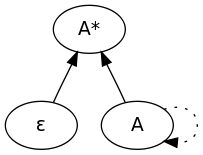
\includegraphics[scale=0.5]{star-list.png}
\caption{GSS representation of a expanded star-list; the solid arrows represent edges and the dotted arrows `next pointers' in the production.}
\end{figure}

These list children can be shared just like any other GSS node. Nothing special needs to be done for this. Since this is the case, worst-case time and space bounds do not change by the introduction of this feature.

Exactly the same principle is used for separated lists and optionals. We will not go into detail on those, since one can easily imagine how these work.

\subsection{Location}

Similar to how lists are implemented, there are also specialized GSS nodes for location related indicators. We have the following varieties:
\begin{enumerate}
 \setlength{\itemsep}{0pt}
 \setlength{\parskip}{0pt}
 \setlength{\parsep}{0pt}
 
 \item Start-of-line
 \item End-of-line
 \item At-column($X$); where $X$ indicates the column number
\end{enumerate}
Basically these are epsilons that only match when we are at a specific location in the input. So they do not consume input and act more like filters then anything else. They can be very useful when parsing certain languages.

\section{Optimizations}
\label{chap:optimizations}

The basic algorithm is fairly straightforward and relatively simple to implement. The naïve implementation will respect worst-case cubic time and space bounds, however adaptations can be made to improve its overall efficiency.

\subsection{General}

\subsubsection{Matching}
A minor performance improvement can be made by matching on entire literals at once, instead of on induvidual characters. This decreases the amount of necessary GSS nodes and thus reduces stack activity, offsetting the performance overhead being scannerless brings along completely.

\subsubsection{Look-ahead}
A more obvious optimization is adding support for look-ahead restrictions. By adding simple checks to the (generated) parser code, we can prevent unnecessary work; if a certain alternative will never match, we do not need to expect it. This both improves performance and will make recognizing / parsing deterministic for LL(k) grammars. When the prefix-sharing optimization (see section \ref{sec:prefixSharing}) is enabled, this will also be the case for LR(k) grammars.

\subsubsection{Breadth-first}
Finally we would like to note that (eventhough it is mandatory for the correctness of our algorithm) a breadth-first general parsing algorithm, or breadth-first implementation of a general parsing algorithm is generally more efficient then a depth-first version. This is because recognizing / parsing can be approached in a level synchronized way, which enables the possibility of handling certain things more efficiently; this mainly has a positive effect on memory usage.

\subsection{Edge related}
\label{sec:edgeOptimizations}

Generally parsers store results on edges in the GSS. If we would refrain from doing this and store parse results elsewhere (in a table with constant look-up time), edges could remain pointers. At first sight this may not be an advantage, however we would be able to share edges among GSS nodes and it opens up numereous other opportunities for optimization.

\subsubsection{Expansion}
\label{subsec:nodeExpansionOptimization}
First of all, by caching `expected children' for every type of node per level a substantial performance increase can be achieved. Additionally, this will ensure linear scaling for non-left-factored grammars. The reason for this is the following; for example, if we take the grammar rules:\\
$S\,::=\,E$\\
$E\,::=\,E + E\,|\,E - E$\\
The expansion at the first level would look like this:
\begin{enumerate}
 \setlength{\itemsep}{0pt}
 \setlength{\parskip}{0pt}
 \setlength{\parsep}{0pt}
 
 \item $.E$ $\rightarrow$ $.E+E$
 \item $.E+E$ edges = \{$.E$\}
 \item $.E$ $\rightarrow$ $.E-E$
 \item $.E-E$ edges = \{$.E$\}
 \item $.E+E$ $\rightarrow$ $.E+E$
 \item $.E+E$ edges = \{$.E$, $.E+E$\}
 \item $.E+E$ $\rightarrow$ $.E-E$
 \item $.E-E$ edges = \{$.E$, $.E+E$\}
 \item $.E-E$ $\rightarrow$ $.E+E$
 \item $.E+E$ edges = \{$.E$, $.E+E$, $.E-E$\}
 \item $.E-E$ $\rightarrow$ $.E-E$
 \item $.E-E$ edges = \{$.E$, $.E+E$, $.E-E$\}
\end{enumerate}
This example clearly demonstrates quardratic behaviour. If we would cache the edges set of one $E$, we could reuse it for any other $E$ in the same level and enable us to update it with additional edges by reference. This is possible since nodes are guaranteed to have the same edges if they are `expected' by the same `parent(s)'. This will make the expansion look like this:
\pagebreak
\begin{enumerate}
 \setlength{\itemsep}{0pt}
 \setlength{\parskip}{0pt}
 \setlength{\parsep}{0pt}
 
 \item $.E$ $\rightarrow$ $.E\,+\,E$
 \item $.E$ $\rightarrow$ $.E\,-\,E$
 \item $E$ edges = \{$.E$\}
 \item $.E+E$ $\Rightarrow$ $E$ edges += $.E+E$
 \item $.E-E$ $\Rightarrow$ $E$ edges += $.E-E$
\end{enumerate}
Now expansion completes in linear time. An additional benefit is that all the edge sets are shared between the children of the different $E$'s, saving memory. It will reduce the worst-case number of edges to $N\,*\,\mathit{numberOfSorts}$. Originally, without sharing, this would have been $N\,*\,\mathit{numberOfProductions}^2$, so this is a massive improvement. One other benefit of this optimization is that it lessens the need for the left-factoring of grammars. In absence of look-ahead filtering expansion performance should be on par with the non-factored equivalent of the grammar; in cases where look-ahead information is used, it may be close enough to remove its necessity.

Also note that this optimization is not only useful in case we have numereous non-factored productions. It also causes the set of edges to be shared between different alternatives associated with the same left-hand-side. So even if we would share the prefixes of all the alternatives (see \ref{sec:prefixSharing}), we would still gain something.

\subsubsection{Reduction}
\label{subsec:edgeVisitOptimization}
As mentioned before, since every GSS node that contains the same non-terminal sort always has the same children if they are in the same level, it is sufficient to initially just follow the first edge in the edge set associated with that level. In case the node this edge points to has already been reduced, nothing needs to be done for this node or any of the other edges in this set (except record the alternative's results, in case we are parsing and not just recognizing); otherwise all other edges in this set need to be followed as normally would have been the case, to queue their associated nodes for reduction. This reduces the number of edge visits significantly.

\subsection{GSS}

\subsubsection{Prefix sharing}
\label{sec:prefixSharing}
In many grammars productions exist that start with the same symbols. There is no reason to do duplicate work for these symbols. For example, if we take the grammar rule: $S\,::=\,E\,+\,E\,|\,E\,-\,E$. Both $E$'s at the start of these productions will always be derived exactly the same way for the same substring(s) and thus they are equal. Because of this, the prefixes of these two productions may as well be merged; i.e. by converting the rule into $S\,::=\,E\,(+\,E\,|\,-\,E)$. It is trivial to modify our algorithm to support this. Simply by allowing every node in the GSS to have more then one `next' node and assigning the same id to both $E$'s (to indicate they must be shared), the desired result can be achieved. Naturally the merged prefixes of grammar rules can be arbitrarily long and are not restricted to just two partially equal rules; as long as a rule's prefix overlaps with another rule it can be merged, regardless whether or not it already has been merged with another rule. This optimization ensures we can recognize and parse LR grammars in linear time. The reason for this is that there will always be one stack at most on which things match, all alternative stacks are guaranteed to die of after visiting each level, thus each visit of a level completes in $O(1)$ time; this leads to the conclusion that the total recognize / parse time for any LR grammar will be $O(N)$, where $N$ is the length of the input.

One may wonder why merging anything other then the prefixes of productions is not supported. While in theory sharing the postfixes of production is also possible, this is more complicated to implement (for reasons we will not elaborate on here) and opportunities to apply this optimization rarely occur in reality. For these reasons we decided not to add this feature to our recognizer / parser. Merging blocks of symbols that are not located at either the beginning or end of productions will never be possible when using our algorithm, since this may lead to incorrect results. For example if we had shared the $B$ of the following alternatives: $S\,::=\,ABC\,|\,DBE$ we would also end up with derivations for $ABE$ and $DBC$, which is obviously undesirable.

\section{Filtering}
\label{chap:filtering}

As is common in general parsing, ultimately you often end up with an ambiguous parse forest. In this chapter we will discuss a number of features we have implemented to filter the trees in this forest. These features are all optional and have no dependencies on eachother.

\subsection{Follow restrictions}

Follow restrictions work as a kind of look-ahead after the production; if the production we are trying to reduce matches the specified character(s) after the current location in the input, the reduce fails. They are mainly, though not exclusively, used to indicate eagerness.

\subsection{Rejects}

Reject filtering is intended for the removal of trees that are not considered to be correct at a certain location in the grammar. One could think of using it for things like filtering alternatives for identifiers that match keywords in the language, for example.

Any alternative of a production can be marked as reject. If this reject alternative matches, all other alternatives this reject belongs to are discarded. In our current implementation, rejected nodes are partially removed from the GSS at parse time and partially during post-parse filtering / flattening. Removing rejected stacks while parsing prevents unnecessary work from being performed; however it can be expensive to do in case the node at the end of a rejected alternative's edge is already reduced. This is the reason why it is not completely done at parse time.

In our current implementation reject rules cannot be nested, since this may lead to incorrect behaviour. Consider the following grammar: $S\,::=\,A(r)\,|\,a,\,A\,::=\,B(r)\,|\,a,\,B\,::=\,a$. The reject alternatives are marked with $(r)$. In this case the order in which reductions are done will determine the final parse result. For example, we could follow the edges from $.a$ to $.A$ and then from $.A(r)$ to $.S$. This will cause $S.$ to be rejected, failing the parse. On the other hand, if we would have followed the edge from $.a$ to $.B$ first and then from $.B(r)$ to $.A$ we would end up with a successful parse, since $A$ gets rejected, preventing the edge from $.A(r)$ to $.S$ from being followed. So if one writes a grammar that contains nested rejects it may, or may not do what was intended.

It is possible to resolve this problem, however this would require a second pass over the tree. Additionally it would prevent us from being able to remove parses that will be filtered in the end, before exploring them further. So it would impact performance in more then one way. This is the main reason why we decided not to support nested reject rules.

\subsection{Priorities and associativity}

Priorities and associativity restrictions are implemented as `don't nest' relations. For example, if we take the grammar rule $E\,::=\,E\,*\,E\,>\,E\,+\,E$, this means that the production $E\,+\,E$ cannot be a child of $E\,*\,E$ on either side of the production. $E\,::=\,E\,+\,E\,\{left\}$ on the other hand means that the production $E\,+\,E$ only cannot be a child of itself on the right side of the production; similarly for $\{right\}$, but the other way around. If declared as $\{nonassoc\}$ it cannot be nested on either side of itself.

The current implementation handles priority and associativity filtering completely at parse time. While reducing, it checks whether or not the reduction is allowed for the edge we want to follow; in case it is, it is stored in a result node that is identified by the sort name of the non-terminal of the node the edge points to and the set of `don't nest' relations associated with this node. This is because the result needs to be shared between all non-terminals with the same sort and `don't nest' relations. For example consider the following grammar rule: $E\,::=\,E * E\,\{left\}\,>\,(E + E\,|\,E - E)\{left\}$. Here $.E + E$ and $.E - E$ would be derived in the same way and thus should share their parse results, just as $E+.E$ and $E-.E$, since their `don't nest' relations are identical.

The main advantage of handling priority and associativity filtering at parse time oppossed to implementing it as post-parse filter is that it is more efficient. We prevent the construction of results that will be thrown away later on, saving memory. Additionally it will prevent unnecessarilly exploring certain parses, because we can determine they will be filtered earlier on, increasing performance.

There is a down-side however. Handling priority and associativity filtering at parse time, disables the edge visit reduction optimization discussed in section \ref{subsec:edgeVisitOptimization}, since we now always need to visit each of the node's outgoing edges at every reduction to check whether or not the nesting is allowed. There is a tradeoff here and it will depend on the grammar whether or not the loss of this optimization can be compensated by what we gain by doing priority and associativity filtering at parse time, opposed to implementing it as a post-parse filter. In our opinion this should be the case for most `real' grammars.

\subsection{Actions}

Each grammar rule can have a number of actions associated with it. These actions can be used to disambiguate non-context-free ambiguities (like C typedefs) or filter alternatives that cannot be disambiguated using priorities. I will not go into detail about this feature, since actions are outside of the scope of this article. The option exists to either intergrate the execution of action into the parser or to apply them as a post-parse filter during, or after, flattening; depending on the requirements or preference of the user. However their implementation is not trivial, because of their interaction with ambiguities and the parse forest.

\section{Benchmarks}

In this chapter we will have a look at the performance of the current Java implementation of our algorithm.

Benchmarks were executed on a machine with the following specifications:
\begin{table}[H]
\centering
\begin{tabular}{ | p{6em} | p{9em} | }
 \hline
 CPU & Intel Q6600 \\
 Memory & 8 GB DDR-800 \\
 OS & Fedora Core 12 \\
 JRE & Sun 1.6.0\_13 (32-bit) \\
 JRE options & -Xmx1800m \\
 \hline
\end{tabular}
\end{table}

Measurements are listed in terms of CPU-time (system + user time) and are gathered using Java's build in management tool. Before performing the benchmarks, the recognizer / parser code was executed a number of times so Java's JIT compiler has the opportunity to optimize.

\subsection{Worst case}

The obvious candidate for a benchmark is the following worst-case grammar:
$S\,::=\,SSS\,|\,SS\,|\,a$\\
input = $a\,*\,50$ to $a\,*\,500$ at $50$ character intervals.

\begin{table}[H]
\centering
\begin{tabular}{ | p{5em} | p{7em} | p{6em} | }
  \hline
  Input chars & Recognize time & Parse time \\
  \hline
  50 & 4 & 6 \\
  100 & 18 & 36 \\
  150 & 60 & 130 \\
  200 & 154 & 332 \\
  250 & 322 & 672 \\
  300 & 596 & 1206 \\
  350 & 996 & 2018 \\
  400 & 1534 & 3184 \\
  450 & 2228 & 4776 \\
  500 & 3090 & 6880 \\
  \hline
\end{tabular}
\caption{Worst-case performance scaling; times are in milliseconds.}
\end{table}

\begin{figure}[H]
\centering
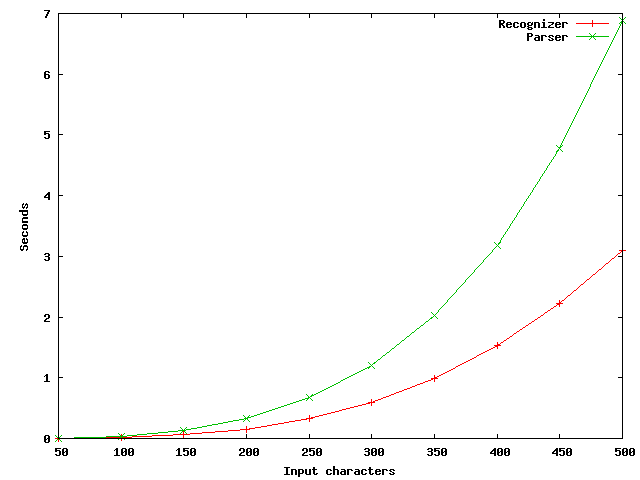
\includegraphics[scale=0.5]{worst-case.png}
\caption{Worst-case recognizer and parser performance scaling.}
\end{figure}

Note however that the recognizer is optimized for speed and the parser for a balance between memory usage and speed (meaning a faster implementation is possible at the cost of increased memory footprint). Regardless of this, our recognizer and parser implementations clearly demonstate cubic worst-case behaviour, as expected. Looking at the times, our implementation seems very efficient in worst-case scenarios.

\subsection{Grammar factoring}

Apart from worst-case behaviour in terms of the number of ambiguous parse results, it is also interesting to look at how well we perform on worst-case grammars without ambiguous input. Here we will compare the performance of our parser between different version of a grammar; a non-factored non-prefix-shared version, a non-factored prefix-shared version and a left-factored version. The original grammar is the following:\\
$S\,::=\,E+$\\
$E\,::=\,a\,|\,E\,+\,E\,|\,E\,-\,E\,|\,E\,*\,E\,|\,E\,/\,E\,|\,E\,>\,E\,|\,...$ 25 more like it ...\\
input = $a\,*\,50000$, $a\,*\,100000$, $a\,*\,150000$ and $a\,*\,200000$

It contains lots of left-recursion and is highly ambiguous; the input, on the other hand, is not ambiguous. Normally one would expect non-linear performance when parsing a string for this grammar. However, as can be seen in the graph below this is not the case. Performance seems to scale perfectly linear regardless of how the grammar is factored.

\begin{figure}[H]
\centering
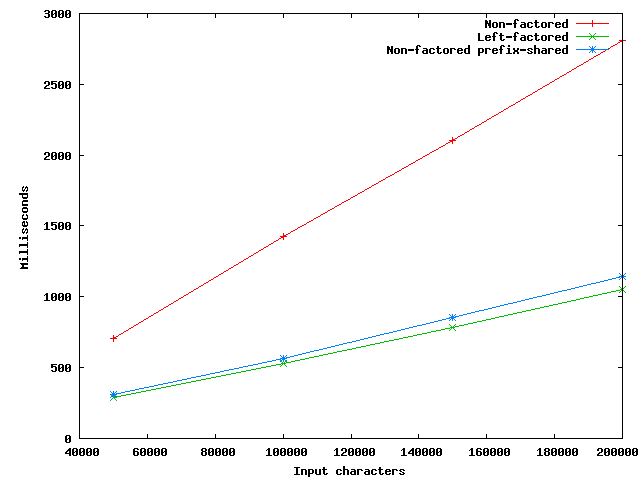
\includegraphics[scale=0.5]{grammar-factoring.png}
\caption{Grammar factoring related parse time scaling; without look-ahead filtering.}
\end{figure}

Note that the parser is about twice as slow on the non-factored non-prefix-shared version of the grammar. This is because both the number of GSS nodes as the number of edge visits is significantly higher for this case. Regardless of this, parsing performance still scales linear with respect to the length of the input, due to the optimization discussed in section \ref{subsec:nodeExpansionOptimization}.

The non-factored prefix-shared and the left-factored versions of the grammar perform almost similar. The main reason that the parser using the left-factored version of the grammar performs better is that our current implementation needs to do a extra work to detect the sharing. However, if required, it is reasonably simple to construct an implementation of our parsing algorithm that does not suffer from this overhead. This is also the reason that look-ahead filtering was disabled for the purposes of this benchmark. If one would enable look-ahead filtering, parsing the left-factored version would become deterministic, since it falls within the LL(1) class of grammars, as the refactoring of the grammar removes all ambiguities from it.

TODO: Add look-ahead filtered left-factored version and fix the text accordingly (shared version will be equivalent in speed and deterministic).

\subsection{Versus non-general}

We also liked to know how we compare when pinned against non-general parsers, since general parsers have the image of being inferior in terms of performance, compared to `normal' LL or LR parsers.

We used the following basic LR grammar for our benchmark:\\
$S ::= E$\\
$E ::= E + F\,|\,F$\\
$F ::= a\,|\,(\,E\,)$\\
input = `$A\,::=\,a\,|\,a+(A)$' from length $100003$, to length $1000003$ at $100000$ character intervals.

We compared our performance results with JavaCup, which was used in combination with JFlex. We selected JavaCup, since it is one of the more widely known and used parser generators that produce LALR parsers in Java.

\begin{figure}[H]
\centering
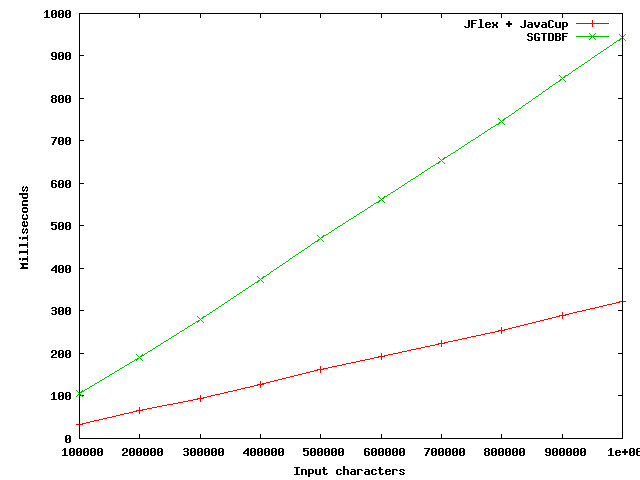
\includegraphics[scale=0.5]{vsLALR.png}
\caption{A parsing performance comparison with a LALR parser.}
\end{figure}

As expected JavaCup performs better. For this specific grammar, JavaCup parses the given input about three times as fast. This seems like a lot, however it is a fairly reasonable result. Especially considering we are using a GSS, since we need to be fully general, instead of the application's stack.

\subsection{Realistic cases}

Benchmarks on artificial grammars are nice for getting a point across or to indicate certain guarantees can be met, however they generally do not offer any insight about performance in realistic cases. Here we will list a number of statistics related to parsing actual source files.

Note that, for now, we just list SDF2 files; a grammar definition format which is mildly ambiguous before filtering. In the future more results will be added for other languages.

\begin{table}[H]
\centering
\begin{tabular}{ | p{5em} | p{5em} | p{6em} | p{10em} |}
  \hline
  Filename & Input & Throughput & Throughput including\\
   & characters & (char/sec) & filtering \& flattening\\
   & & & (char/sec)\\
  \hline
  ATerm.def & 2393 & 341857 & 217545\\
  C.def & 10552 & 363862 & 245395\\
  SDF2.def & 18054 & 368448 & 234467\\
  Java.def & 30983 & 360267 & 232954\\
  \hline
\end{tabular}
\caption{Average parser throughput.}
\end{table}

\pagebreak
One does have to take into account that our current implementation is written in Java. If we would re-implement it in C, a performance increase of at least three to five fold is to be expected. Putting our throughput at around 1 million characters per second, while having all filters enabled, in the SDF2 case.

Regardless of this, compared to the parser we previously used, a C implementation of scannerless GLR, we achieved a performance gain of roughly 40\% (i.e. our implementation parses the same file in 0.6 the amount of time), in this specific case.

\section{Prototype}

The development of this algorithm was approached in a rather unorthodox way. Rather then starting with the design of the algorithm and making an implementation for validation and testing purposes afterwards, we started with implementing a basic top-down recognizer, extending it to a parser, followed by testing, profiling and optimization; gradually we improved this implementation and its algorithm, until it matched our requirements. By using this approach we are able to get more direct feedback about issues and scalability and performance bottlenecks. Additionally opportunities for optimization will be highlighted that may not be immediately apparent or which may be overlooked when looking at the problem from a purely algorithmic point of view.

The main purpose of this project has always been to create a working, usable general parser implementation. The development of a new algorithm was secondary but required, since no suitable alternative was available for our purposes.

Our first implementation is written in Java. The reason we chose this language for our prototype was that is was both required for our current project and gave us the opportunity to easily change and extend it. The down side is that it makes is harder to make a comparison with other general parser implementations, which are mainly written in C and thus have a major performance advantage.

\pagebreak
\section{Future work}

Numereous things can still be improved or changed. Mostly these involve optimizations or implementation improvements. We will not go into detail, but just list a number of ideas instead.

\begin{enumerate}
 \setlength{\itemsep}{0pt}
 \setlength{\parskip}{0pt}
 \setlength{\parsep}{0pt}
 
 \item Prefix sharing can be implemented more efficiently by moving more logic to the generator, so parts of productions do not have to be merged dynamically any more.
 \item We can pre-construct a data structure which contains sort to alternatives mappings in combination with their look-ahead information, so we can obtain relevant alternatives more efficiently.
 \item Nullable derivations or trees can be pre-computed or dynamically cached, improving efficiency.
 \item Matching could be handled more efficiently (more bottom-up like, so we `touch' less terminals).
 \item Pre-computed information about priority / associativity restrictions can be used to handle filtering more efficiently.
 \item Some rejects can be statically computed and used as a kind of `disallowed' look-ahead. This prevents alternatives of which we know they will die in advance from being explored.
 \item Multi-core / processor support is relatively easy to add and may be interesting to explore as possible performance booster for certain cases.
\end{enumerate}

Finally, it would be interesting to create a C implementation of our parsing algorithm, both to see how far we can push the parser's throughput and to be able to make a broader and more accurate performance comparison with implementations of other (general) parsing algorithms. We expect to do fairly well in such a showdown.

\section{Conclusion}

In this article we described our parsing algorithm, discussed optimizations that can be applied to it and gave an impression of its capabilities. To summarize, we developed a general parsing algorithm that is both easy to comprehend and scales well, regardless of the input or grammar used. The best of both worlds, combined into one beautiful, elegant solution.

\pagebreak
\section{References}

TODO:\\
-GSS\\
-LL\\
-LR\\
-SPPF (and binarized)\\
-GLR\\
-SGLR (and ASF+SDF-Meta)\\
-JFlex\\
-JavaCup\\
-SDF2

\end{document}
